%%=============================================================================
%% Supplementary Materials for the MDPI *Mathematics* submission
%%   "An End-to-End Multimodal System for Subtitle Recognition and
%%    Chinese-Japanese Translation with Speech Synthesis in Short Dramas"
%%
%% >>> COMPILE WITH XeLaTeX <<<  (contains Chinese/Japanese characters via xeCJK).
%% This is a standalone document (compiles on its own); when submitting to MDPI
%% you may either upload the compiled PDF as "Supplementary Materials" or paste
%% the content into the MDPI supplementary template. Tables/figures are numbered
%% S1, S2, ... per MDPI supplementary convention.
%%=============================================================================
\documentclass[11pt]{article}
\usepackage[a4paper,margin=2.2cm]{geometry}
\usepackage{amsmath,amssymb,amsfonts}
\usepackage{graphicx}
\usepackage{booktabs}
\usepackage{array}
\usepackage{algorithm}
\usepackage{algpseudocode}
\usepackage{pgfplots}
\pgfplotsset{compat=1.18}
\usepackage{xeCJK}
\setCJKmainfont{Noto Serif CJK SC}

% S-prefixed numbering for supplementary floats
\renewcommand{\thetable}{S\arabic{table}}
\renewcommand{\thefigure}{S\arabic{figure}}
\renewcommand{\thealgorithm}{S\arabic{algorithm}}
\renewcommand{\theequation}{S\arabic{equation}}

\title{\vspace{-1.5em}Supplementary Materials:\\ An End-to-End Multimodal System for Subtitle Recognition and\\ Chinese--Japanese Translation with Speech Synthesis in Short Dramas}
\author{Jing An, Qiming Bao, and Jinhua Su}
\date{}

\begin{document}
\maketitle
\vspace{-1.5em}
\noindent This document collects supporting tables, figures, and the fusion pseudocode referenced from the main manuscript. Numbering is independent of the main paper.

\begin{algorithm}[t]
\caption{Confidence-Adaptive OCR/ASR Fusion}
\label{alg:fusion}
\begin{algorithmic}[1]
\Require Whisper segments $\mathcal{A}$, OCR detections $\mathcal{O}$, time tolerance $\delta$, log-prob threshold $\theta_p$, similarity threshold $\theta_s$
\Ensure Fused subtitle sequence $\mathcal{S}$
\State $\mathcal{S} \gets \emptyset$
\For{each $a_i = (t_i^s, t_i^e, w_i, p_i) \in \mathcal{A}$}
    \State $\mathcal{C}_i \gets \{\, o_j \in \mathcal{O} \mid \tau_j \in [t_i^s - \delta,\; t_i^e + \delta]\,\}$ \Comment{candidate OCR detections}
    \If{$p_i \geq \theta_p$} \Comment{ASR is confident; trust Whisper}
        \State $\hat{w}_i \gets w_i$
    \Else
        \State $o^\star \gets \arg\max_{o_j \in \mathcal{C}_i}\, \mathrm{sim}(o_j, w_i)$ \Comment{best OCR match}
        \If{$\mathcal{C}_i \neq \emptyset$ \textbf{and} $\mathrm{sim}(o^\star, w_i) \geq \theta_s$}
            \State $\hat{w}_i \gets o^\star$ \Comment{substitute OCR text, retain ASR timing}
        \Else
            \State $\hat{w}_i \gets w_i$ \Comment{fallback: keep ASR}
        \EndIf
    \EndIf
    \State $\mathcal{S} \gets \mathcal{S} \cup \{(t_i^s, t_i^e, \hat{w}_i)\}$
\EndFor
\State \Return $\mathcal{S}$
\end{algorithmic}
\end{algorithm}

\begin{table}[t]
\centering
\caption{Statistical information of the proposed dataset.}
\label{tab:dataset}
\begin{tabular}{lrlr}
\toprule
\multicolumn{2}{c}{\textbf{Dataset Composition}} & \multicolumn{2}{c}{\textbf{Subtitle Statistics}} \\
\cmidrule(lr){1-2} \cmidrule(lr){3-4}
Video clips (total) & 82 & Total duration (min) & 130.56 \\
Paired episodes & 79 & Subtitle segments & 3{,}692 \\
Speaker IDs & 12 & Avg. segments/episode & 46.7 \\
\bottomrule
\end{tabular}
\end{table}

\begin{table}[t]
\centering
\caption{Gating-rule ablation under a single unified evaluation harness (identical fusion implementation and corpus-level segment-joined metrics; all 79 episodes). ``Static'' rows open the log-probability gate for every segment ($\theta_p{=}0$); the Adaptive row applies the selected operating point ($\theta_p{=}-0.2$, $\theta_s{=}80$). All rows are directly comparable. Absolute values differ from the production-pipeline fusion metrics in the main paper due to the corpus-level text-joining format. Best per column in bold.}
\label{tab:fusion_ablation}
\begin{tabular}{lccccc}
\toprule
\textbf{Fusion Strategy} & \textbf{BLEU}$\uparrow$ & \textbf{chrF++}$\uparrow$ & \textbf{CER}$\downarrow$ & \textbf{CharAcc}$\uparrow$ & \textbf{Comp.}$\uparrow$ \\
\midrule
Never Replace (ASR only)         & 81.31 & 67.20 & \textbf{0.156} & 0.898 & 0.8066 \\
Always Replace ($\theta_s{=}0$)  &  0.51 & 14.07 & 0.872 & 0.138 & 0.1030 \\
Static ($\theta_s{=}40$)         & 81.35 & \textbf{68.32} & 0.161 & \textbf{0.901} & 0.8091 \\
Static ($\theta_s{=}60$)         & 81.48 & 68.12 & 0.158 & 0.900 & \textbf{0.8094} \\
Static ($\theta_s{=}80$)         & \textbf{81.61} & 67.77 & \textbf{0.156} & 0.899 & 0.8092 \\
\midrule
Adaptive ($\theta_p{=}-0.2$, $\theta_s{=}80$, ours) & 81.60 & 67.73 & \textbf{0.156} & 0.899 & 0.8091 \\
\bottomrule
\end{tabular}
\end{table}

\begin{figure}[t]
\centering
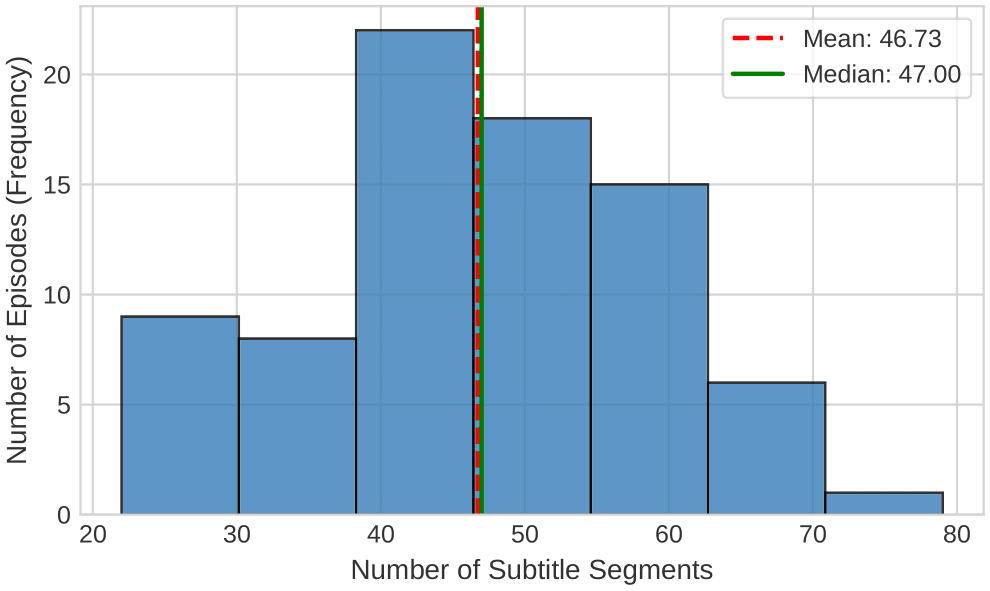
\includegraphics[width=0.7\textwidth]{fig_2.png}
\caption{Distribution of subtitle segments per episode across the 79-episode dataset.}
\label{fig:subtitle_dist}
\end{figure}

\begin{table}[t]
\centering
\caption{Frame sampling rate ablation for subtitle recall on episode 11.mp4 using Qwen3-VL-4B.}
\label{tab:fps_ablation}
\begin{tabular}{lcc}
\toprule
\textbf{Sampling Rate} & \textbf{Detected Characters} & \textbf{Recall vs.\ 5\,fps} \\
\midrule
1\,fps & 411 & 27.7\% \\
2\,fps & 659 & 44.3\% \\
5\,fps & 1{,}486 & 100\% (upper bound) \\
\bottomrule
\end{tabular}
\end{table}

\begin{table}[t]
\centering
\caption{Grid search composite scores on the 20-episode validation set. Each cell is the corpus-level composite score for the fusion strategy gated by $(\theta_p, \theta_s)$. The upper-left ``flat'' region ($\theta_p \leq -0.8$) corresponds to the ASR-always regime: only 1.6\% of corpus segments have avg\_logprob below $-0.8$, so essentially no OCR substitutions occur. Scores are rounded to three decimal places; the bold marks the unique full-precision maximum ($\theta_p{=}-0.2$, $\theta_s{=}80\%$: 0.8051 vs.\ 0.8046 at $\theta_s{\in}\{40\%,70\%\}$, which also round to 0.805).}
\label{tab:param_grid}
\begin{tabular}{c|ccccc}
\toprule
$\theta_p$ \textbackslash\ $\theta_s$ & 40\% & 50\% & 60\% & 70\% & 80\% \\
\midrule
$\leq -0.8$ & 0.800 & 0.800 & 0.800 & 0.800 & 0.800 \\
$-0.5$      & 0.802 & 0.801 & 0.800 & 0.800 & 0.800 \\
$-0.4$      & 0.802 & 0.801 & 0.800 & 0.800 & 0.800 \\
$-0.3$      & 0.804 & 0.803 & 0.802 & 0.802 & 0.803 \\
$-0.2$      & 0.805 & 0.803 & 0.803 & 0.805 & \textbf{0.805} \\
\bottomrule
\end{tabular}
\end{table}

\begin{table}[t]
\centering
\caption{Word-level error type analysis of adaptive fusion corrections (jieba POS; nr/ns/nt/nz = proper nouns). GT correction rate: fraction of substitutions that moved the output closer to the ground truth.}
\label{tab:error_type}
\begin{tabular}{lrrrr}
\toprule
\textbf{Category} & \textbf{Substitutions} & \textbf{\% of Total} & \textbf{GT Corrections} & \textbf{Correction Rate} \\
\midrule
Proper nouns (nr/ns/nt/nz) &  30 & 13.2\% & 18 & \textbf{60.0\%} \\
Numbers                    &   4 &  1.8\% &  3 & 75.0\% \\
Common vocabulary          & 193 & 85.0\% & 114 & 59.1\% \\
\midrule
\textbf{Total}             & \textbf{227} & & & \\
\bottomrule
\end{tabular}
\end{table}

\begin{figure}[t]
\centering
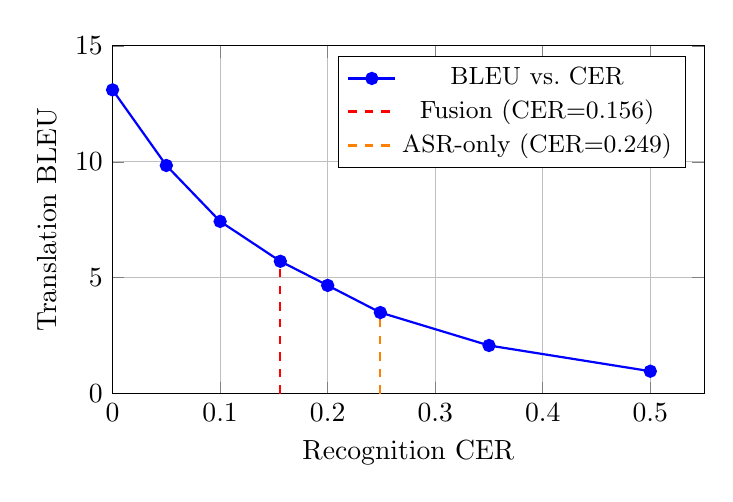
\begin{tikzpicture}
\begin{axis}[
  xlabel={Recognition CER},
  ylabel={Translation BLEU},
  width=0.75\textwidth, height=6cm,
  xmin=0, xmax=0.55,
  ymin=0, ymax=15,
  grid=major,
  legend pos=north east,
  legend style={font=\small},
  mark size=2pt,
]
\addplot[blue, mark=*, thick] coordinates {
  (0.000,13.10)(0.050,9.84)(0.100,7.43)
  (0.156,5.71)(0.200,4.67)(0.249,3.50)
  (0.350,2.08)(0.500,0.97)
};
\addplot[red, dashed, thick] coordinates {(0.156,0)(0.156,5.71)};
\addplot[orange, dashed, thick] coordinates {(0.249,0)(0.249,3.50)};
\legend{BLEU vs.\ CER, Fusion (CER=0.156), ASR-only (CER=0.249)}
\end{axis}
\end{tikzpicture}
\caption{Cross-stage error propagation: translation BLEU as a function of recognition CER. Dashed lines mark the operating points of ASR-only (CER=0.249) and Adaptive Fusion (CER=0.156). The fusion's recognition improvement yields +2.2 BLEU in the translation stage.}
\label{fig:error_prop}
\end{figure}

\begin{table}[t]
\caption{End-to-end pipeline evaluation on 16 fold-0 validation episodes. Source text fed to the Qwen3-VL-4B LoRA translation model varies by condition; metrics are computed at the document level (entire episode as one unit) against the Japanese ground truth. chrF++ is the primary metric (character-level, more robust than BLEU for Japanese at document granularity). The ASR-only BLEU of 0.00 is a genuine consequence of propagated proper-noun errors eliminating all document-level 4-gram matches, not an evaluation artefact (see main text).}
\label{tab:e2e}
\centering
\begin{tabular}{lcc}
\toprule
\textbf{Source Condition} & \textbf{BLEU}$\uparrow$ & \textbf{chrF++}$\uparrow$ \\
\midrule
Oracle (gold Chinese text)   & 5.02 & 14.97 \\
Adaptive Fusion (ours)       & 0.48 & 13.56 \\
ASR-only (Whisper-medium)    & 0.00 & 11.32 \\
\bottomrule
\end{tabular}
\end{table}

\begin{table}[t]
\centering
\caption{Translation quality ablation: visual context vs.\ text-only input using Qwen3-VL zero-shot on 20 episodes. Absolute BLEU gain: +3.35.}
\label{tab:ablation_context}
\begin{tabular}{lcc}
\toprule
\textbf{Input Modality} & \textbf{BLEU}$\uparrow$ & \textbf{chrF++}$\uparrow$ \\
\midrule
Text-Only (OCR subtitles)       & 10.09 & 28.26 \\
Multimodal (Video frames + Text) & \textbf{13.44} & \textbf{29.70} \\
\bottomrule
\end{tabular}
\end{table}

\begin{table}[t]
\centering
\caption{TTS reference audio duration ablation using F5-TTS. Speaker similarity measured via cosine similarity of speaker embeddings.}
\label{tab:ablation_tts}
\begin{tabular}{lc}
\toprule
\textbf{Reference Duration} & \textbf{Speaker Similarity}$\uparrow$ \\
\midrule
Short ($\sim$3\,s) & 0.64 \\
Long ($\sim$10\,s) & \textbf{0.71} \\
\bottomrule
\end{tabular}
\end{table}

\begin{table}[t]
\centering
\caption{Qualitative translation examples. Example A shows a culturally nuanced term translated correctly by FT but incorrectly by ZS. Example B shows an OOV-driven hallucination by FT that ZS avoids.}
\label{tab:qual_examples}
\begin{tabular}{llp{3.6cm}p{3.6cm}p{3.2cm}}
\toprule
\textbf{Ex.} & \textbf{Chinese source} & \textbf{FT (ours)} & \textbf{ZS (Qwen3-VL-4B)} & \textbf{Reference} \\
\midrule
A & 看来我们挺有缘 & \textbf{きっと縁があるな} \newline (cultural term preserved) & きっと運が良いのだろう \newline (semantic error: 縁→運) & やっぱり縁があるのかもね \\
\midrule
B & 拜托 & お前はお母さんも有名なファッションデザイナーのWhiteさんだろ \newline (OOV hallucination) & お祈り & っていうか \\
\bottomrule
\end{tabular}
\end{table}

\end{document}
